\chapter{Test a guitars output impedance}\label{app:output_impedance}
A test was made to get a view of the output impedance of a guitar.

\section*{Materials and setup}
To measure the output impedance on a guitar, the following materials are used:
\begin{itemize}
\item Digilent Analog Discovery 2 (Oscilloscope)
\item Fender Squier Classic Vibe Telecaster (Guitar)
\item Digilent Waveforms 2015 (PC - software)
\end{itemize}

\begin{figure}[htbp!]
\centering
\begin{picture}(0,0)%
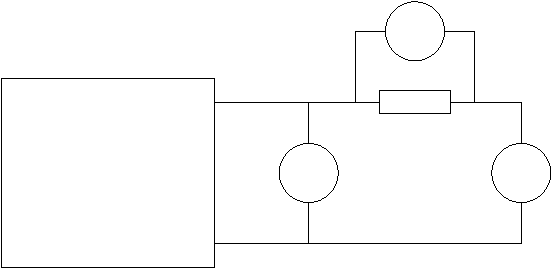
\includegraphics{guitar_output_impedance.pdf}%
\end{picture}%
\setlength{\unitlength}{4144sp}%
%
\begingroup\makeatletter\ifx\SetFigFont\undefined%
\gdef\SetFigFont#1#2#3#4#5{%
  \reset@font\fontsize{#1}{#2pt}%
  \fontfamily{#3}\fontseries{#4}\fontshape{#5}%
  \selectfont}%
\fi\endgroup%
\begin{picture}(4205,2045)(4129,-2773)
\put(7561,-871){$-$}%
\put(6346,-1996){$Osc$}%
\put(6346,-2176){$Ch2$}%
\put(7156,-916){$Osc$}%
\put(7156,-1096){$Ch1$}%
\put(7966,-1996){$Osc$}%
\put(8011,-2176){$W1$}%
\put(7066,-1591){$R$}%
\put(4681,-2086){$Guitar$}%
\put(6346,-1771){$+$}%
\put(6346,-2401){$-$}%
\put(6931,-871){$+$}%
\end{picture}%
\caption{Setup for measuring output impedance on a guitar.}
		\label{fig:appendix:guitar_output_impedance}
\end{figure}

\section*{Test procedure}


\begin{enumerate}
\item The materials are set up as in \autoref{fig:appendix:guitar_output_impedance}.
\item The Digilent Waveform 2015 is set as a Network analyser.
\item  The guitar is set to use the neck pickup and the volume and tone control are tuned all the way up
\item  The network analyser is set to measure $V_{peak}$ from \SI{10}{\hertz} to \SI{22}{\kilo\hertz} with 5000 sample and the resistor R is chosen to \SI{10}{\kilo\ohm}
\item The measured data on the Osc ch1 and ch2 is used in the following formula $\left | Z_o \right | = \frac{V_{Ch1}}{V_{Ch2}}\cdot R$ which depend on the frequency. 
\item The same procedure is done on the bridge pickup, and with both neck and bridge pickup i activated.
\item The data is plotted in MATLAB
\end{enumerate}

\section*{Results}

\begin{figure}[htbp!]
	\centering
		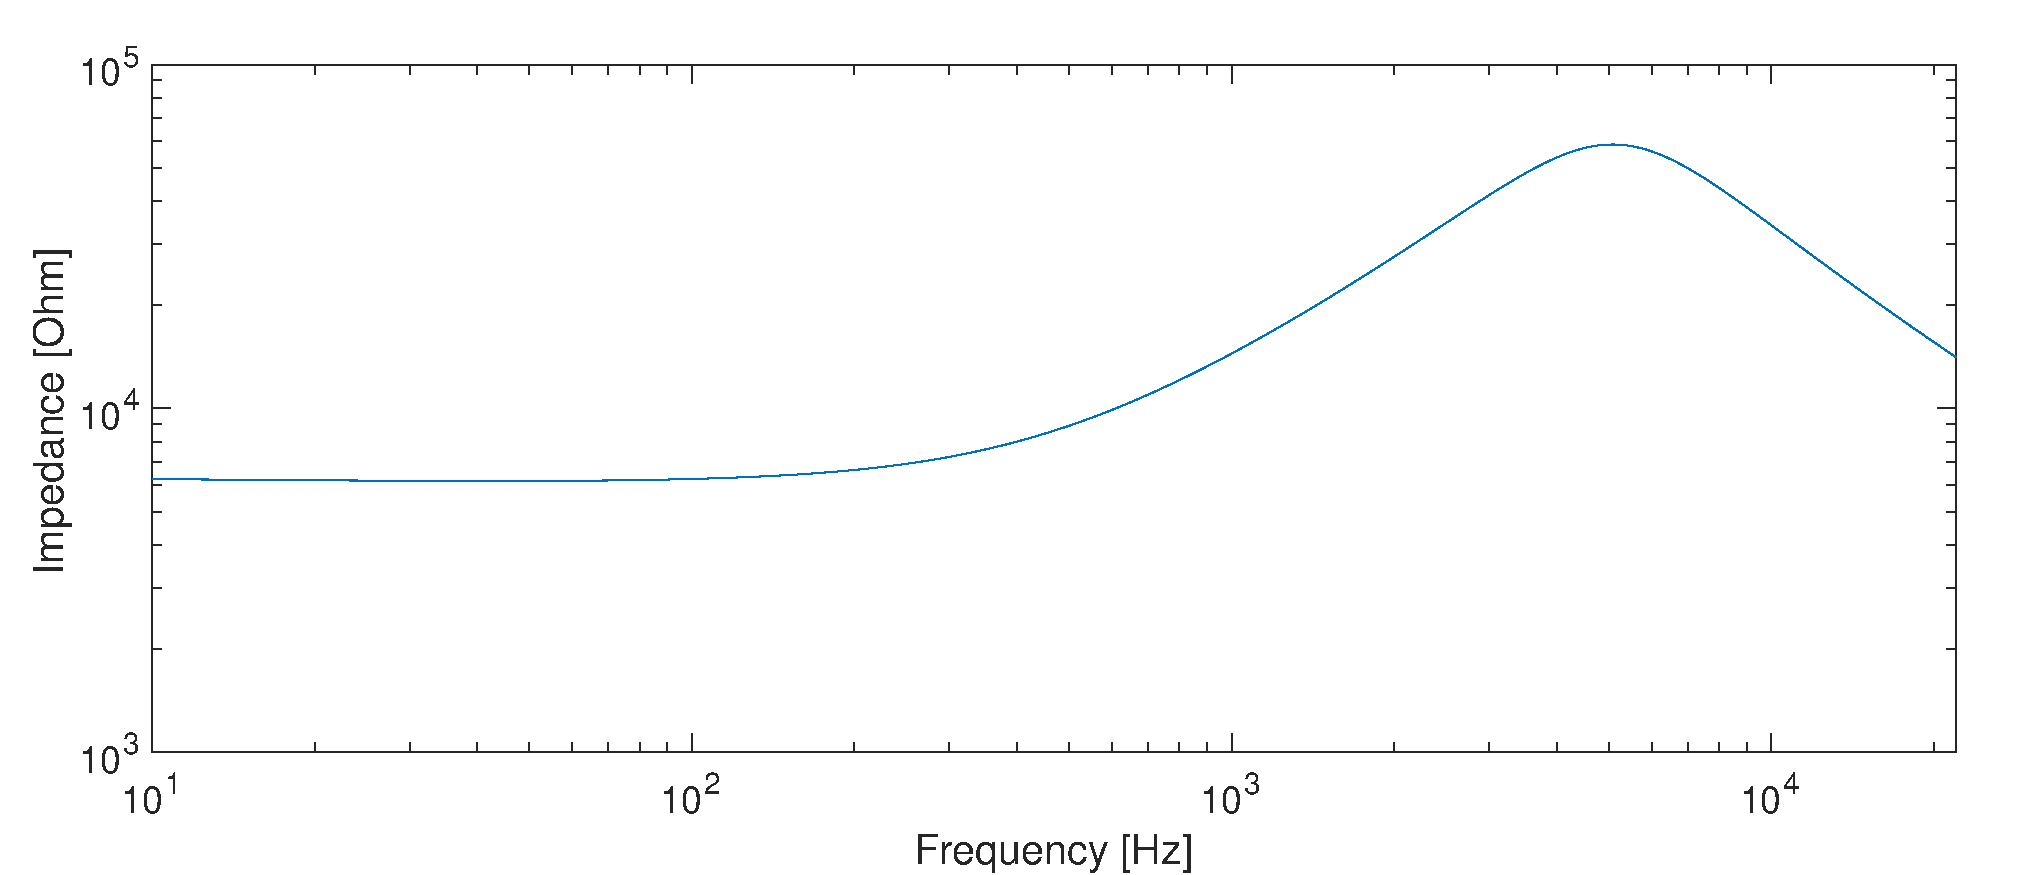
\includegraphics[width=1\textwidth]{guitar_neck_picup.pdf}
		\caption{Measurement of the output impedance of the neck pickup.}
		\label{fig:appendix:guitar_neck_picup}
\end{figure}

On \autoref{fig:appendix:guitar_neck_picup} it is seen that the output impedance is lowest at \SI{10}{\hertz} with \SI{6220}{\ohm}  and the highest output impedance is \SI{58,51}{\kilo\ohm} at \SI{5167}{\hertz}, and afterwords the impedance is failing until the stop point at \SI{22}{\kilo\hertz}.

\begin{figure}[htbp!]
	\centering
		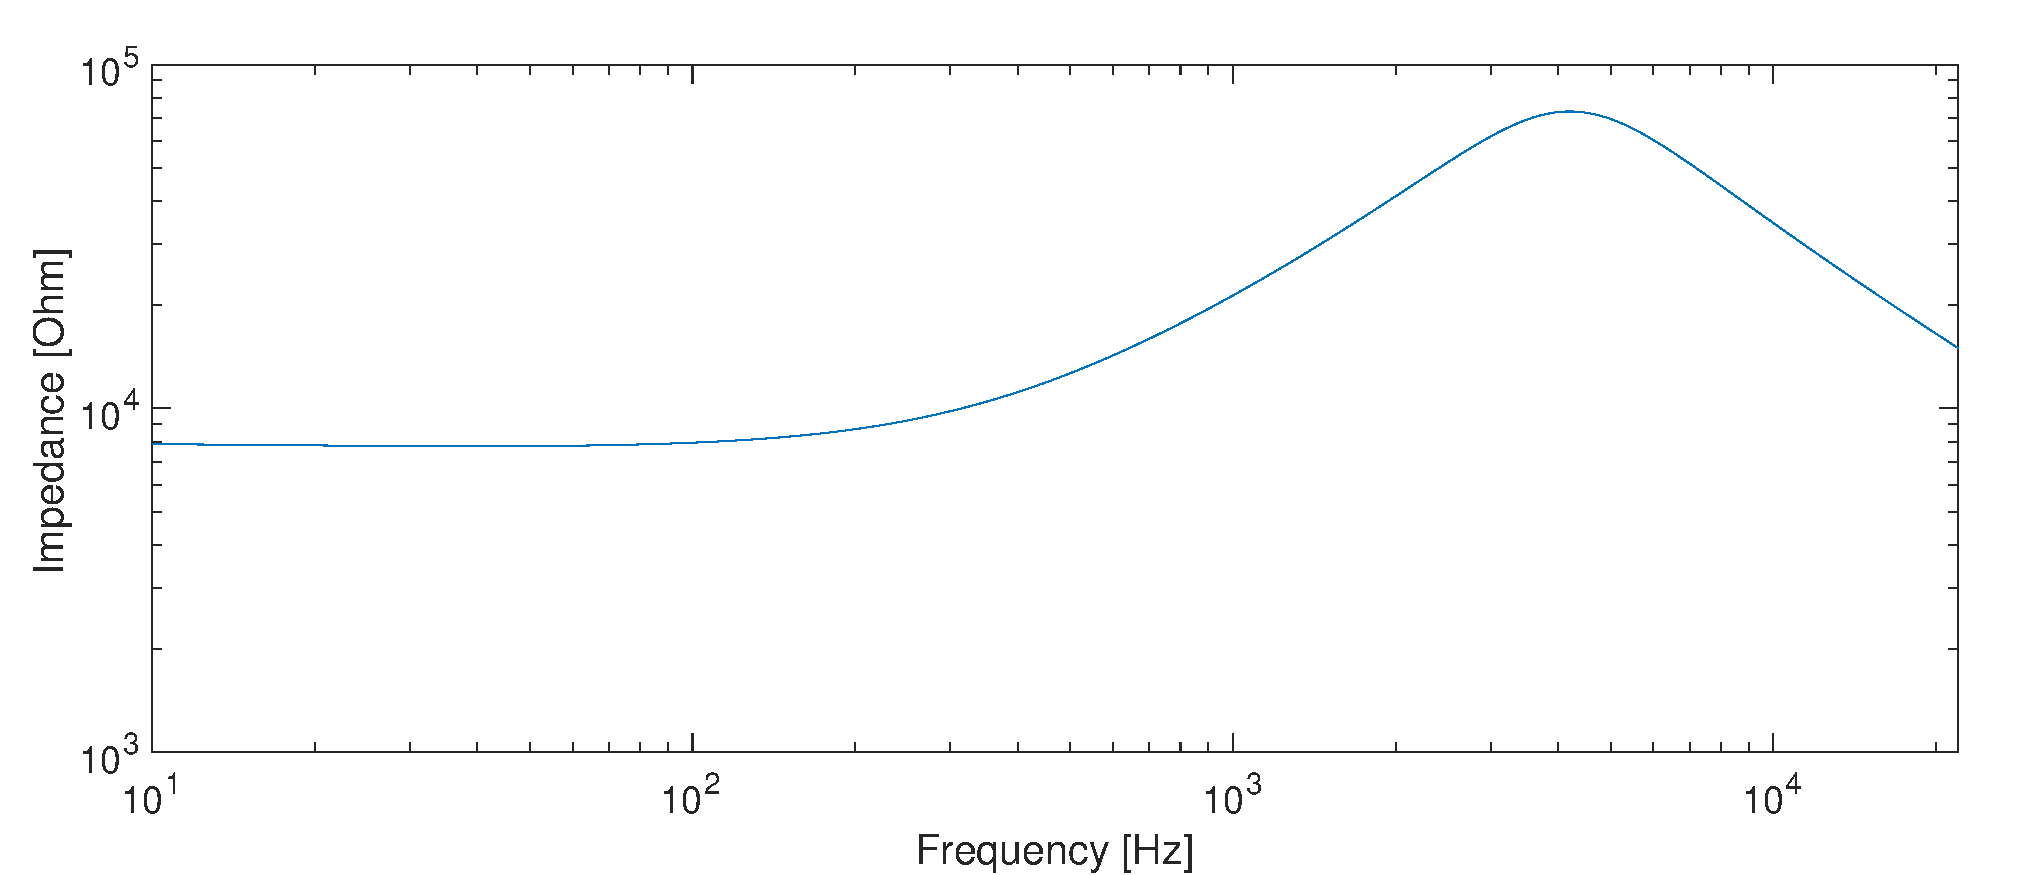
\includegraphics[width=1\textwidth]{guitar_bridge_picup.pdf}
		\caption{Measurement of the output impedance of the bridge pickup.}
		\label{fig:appendix:guitar_bridge_picup}
\end{figure}

On  \autoref{fig:appendix:guitar_bridge_picup} it is seen that the output impedance is lowest at \SI{10}{\hertz} with \SI{7863}{\ohm}  and the highest output impedance is \SI{73,06}{\kilo\ohm} at \SI{4010}{\hertz}, and afterwords the impedance is failing until the stop point at \SI{22}{\kilo\hertz}.

\begin{figure}[htbp!]
	\centering
		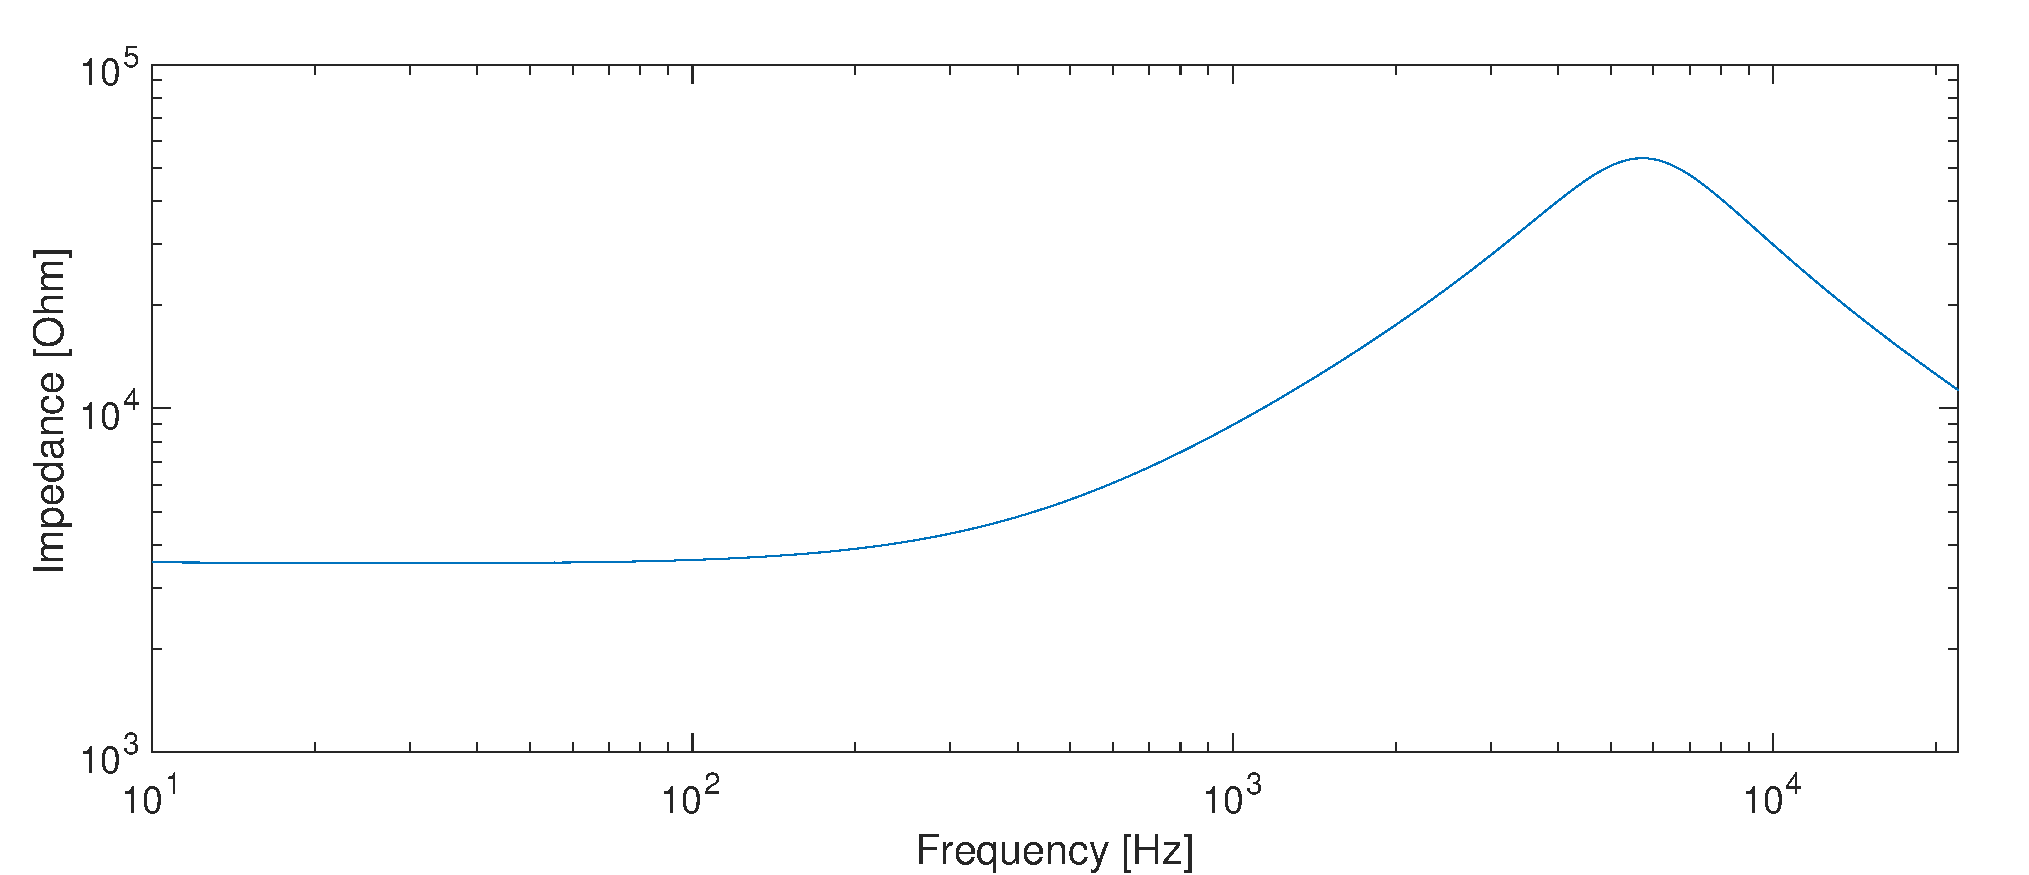
\includegraphics[width=1\textwidth]{guitar_neck_and_bridge_picup.pdf}
		\caption{Measurement of the output impedance of the neck and bridge pickup in parallel.}
		\label{fig:appendix:guitar_neck_and_bridge_picup}
\end{figure}

On  \autoref{fig:appendix:guitar_neck_and_bridge_picup} it is seen that the output impedance is lowest at \SI{10}{\hertz} with \SI{3563}{\ohm}  and the highest output impedance is \SI{53,43}{\kilo\ohm} at \SI{5702}{\hertz}, and afterwords the impedance is failing until the stop point at \SI{22}{\kilo\hertz}.